\documentclass[a4paper]{jpconf}
\bibliographystyle{iopart-num}
\usepackage{amsmath}
\usepackage{citesort}
\usepackage{subfigure}
\usepackage{graphicx}
\graphicspath{{fig/}}
\usepackage{ifpdf}
\ifpdf\usepackage{epstopdf}\fi
\usepackage[export]{adjustbox}

%----------------------------------------------------- 
%\usepackage{soul,ulem,color,xspace,bm}
% Andrei's commands
% Suggest to remove
%\newcommand{\asrm}[1]{{\color{magenta}\sout{#1}}}
% Suggest to insert
%\newcommand{\as}[1]{\color{cyan}#1\xspace\color{black}}
% Suggest to replace
%\newcommand{\asrp}[2]{\asrm{#1} \as{#2}}
% Comment
%\newcommand{\ascm}[1]{{\color{green}\;AS: #1}}
%------------------------------------------------------

\begin{document}
\title{Electron and ion acceleration by relativistic shocks: particle-in-cell model simulations}

\author{V I Romansky$^{1,2}$, A M Bykov$^{1,3}$ and S M Osipov$^1$}

\address{$^1$ Ioffe Institute, 26 Politekhnicheskaya st., St. Petersburg 194021, Russia}
\address{$^2$
	Sternberg Astronomical Institute, Moscow State University
	Universitetsky pr., 13, Moscow 119234, Russia}
\address{$^3$ Peter the Great St.~Petersburg Polytechnic University, 29 Politekhnicheskaya st., St. Petersburg 195251, Russia}

\ead{romanskyvadim@gmail.com}

\begin{abstract}
	The problem of particle acceleration by the collisionless astrophysical shocks is of fundamental importance for the cosmic ray origin problem and the high energy astrophysics. The fast magnetohydrodynamical shocks produced by relativistic jets are considered as the very likely sites of the cosmic ray acceleration.
	While cosmic ray acceleration by both non-relativistic and ultra relativistic shocks was studied in some details the shocks of a moderate Lorentz factors has attracted much less attention so far, while they are important for modelling the gamma-ray burst afterglows and a number of other interesting objects. In this paper we present the results of simulations of relativistic shock waves in the electron-proton plasmas obtained with an implicit particle-in-cell code for the initial study the particle injection efficiencies.
\end{abstract}
\section{Introduction}
One of the possible sources of high-energy cosmic rays are shock waves in astrophysical collisionless plasma due to the diffusive shock acceleration (DSA) mechanism, see \cite{Bell1978}, \cite{Blandford1978}. Strong magnetic fields are necessary for effective acceleration of charged particles and the observations of the synchrotron emission from supernova remnants (SNRs) show, that the magnetic field there is about 100 times stronger then the interstellar field (see for example \cite{Berezhko2003},\cite{Uchiyama2007}). So strong fields can be produced due to instabilities in anisotropic plasma. One of the most powerful methods to explore processes in collisionless plasma is the Particle-in-Cell simulation. In this work we explore instabilities in the plasma using this method. 
We developed the implicit particle-in-cell (PIC) code, based on the scheme suggested by Lapenta et al.~\cite{Lapenta2006} and improved for the relativistic case by Noguchi et al.\cite{Noguchi2007}.
Our code is fully three dimensional and parallelized with MPI technology, which is adapted for distributed computing and can be executed on a wide class of computers.
\section{Shock wave simulation}
We studied the evolution of trans-relativistic shocks and spectum of accelerated particles. We chose relastivistic shocks with low lorenz-factor because the maximum energy of produced cosmic rays increases with shock wave lorenz-factor, but the efficiency of acceleration decreases, because it is more difficult for particle to cross fast moving front many times \cite{Ellison2013}. So we assume that intermediate case of trans-relativistic shocks provides the most effective acceleration.

We developed the implicit particle-in-cell (PIC) code, based on the scheme suggested by Lapenta et al.~\cite{Lapenta2006} and improved for the relativistic case by Noguchi et al.\cite{Noguchi2007}.
Our code is fully three dimensional and parallelized with MPI technology, which is adapted for distributed computing and can be executed on a wide class of computers.

In simulation setup the homogeneous plasma, which flows in through the right boundary
and collides with the reflecting superconducting wall on the left boundary. 
  
 Simulations are one-dimensional and have following parameters: initial flow lorenz-factor $\gamma = 1.5$, number densities $n_e = 10^{-4} \rm{cm}^{-3}$, $n_p = 10^{-4} \rm{cm}^{-3}$ , temperature $5\cdot10^8 \rm{K}$, magnetic field $B = 10^{-4} \rm{G}$, the full size of the box $L = 4\cdot10^{12} \rm{cm}$, the number of cells $N=4\cdot10^4$. Electron mass is reduced to $m_e = \frac{m_p}{20}$. The full time of simulation is $T = 5000 {\omega_p}^{-1}$. $\theta$ is angle between flow velocity and magnetic field. We present results of particle spectrum in several simulations with different $\theta$. 
\begin{figure}[h!]
	\centering
	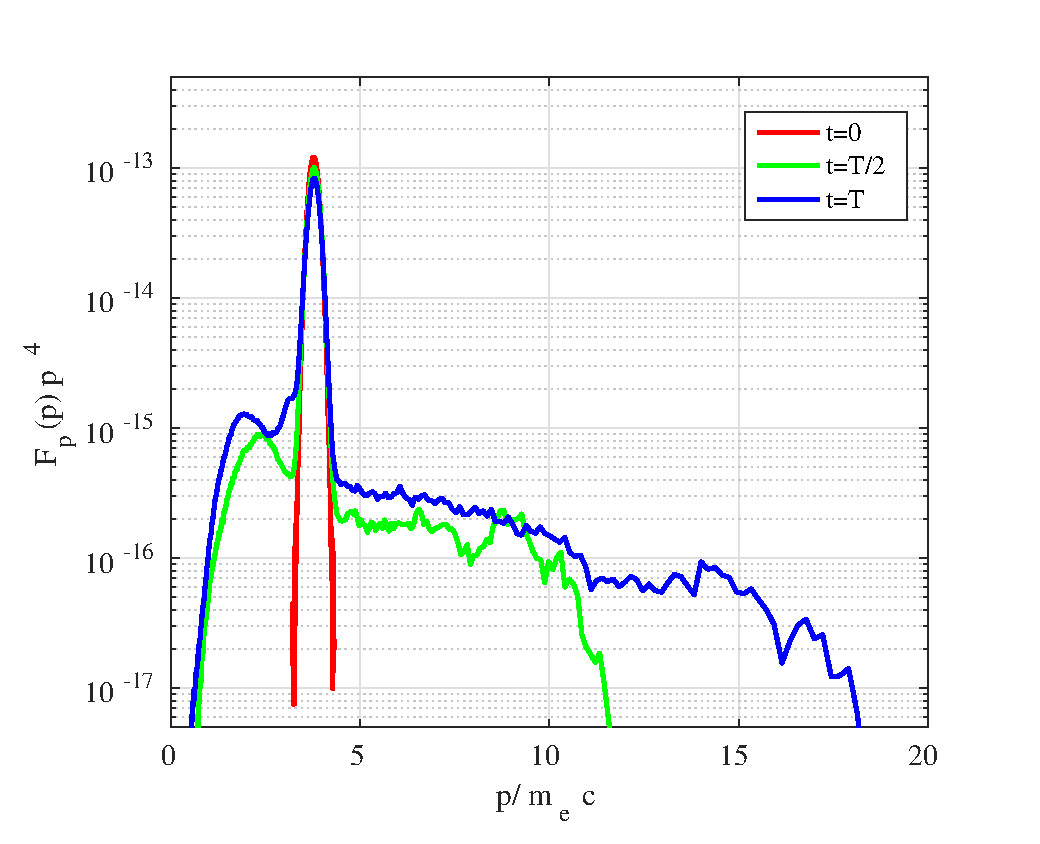
\includegraphics[width=0.8\textwidth]{fig/protons.eps} 
	\caption{Distribution of protons.}
	\label{protons}
\end{figure}
\begin{figure}[h!]
	\centering
	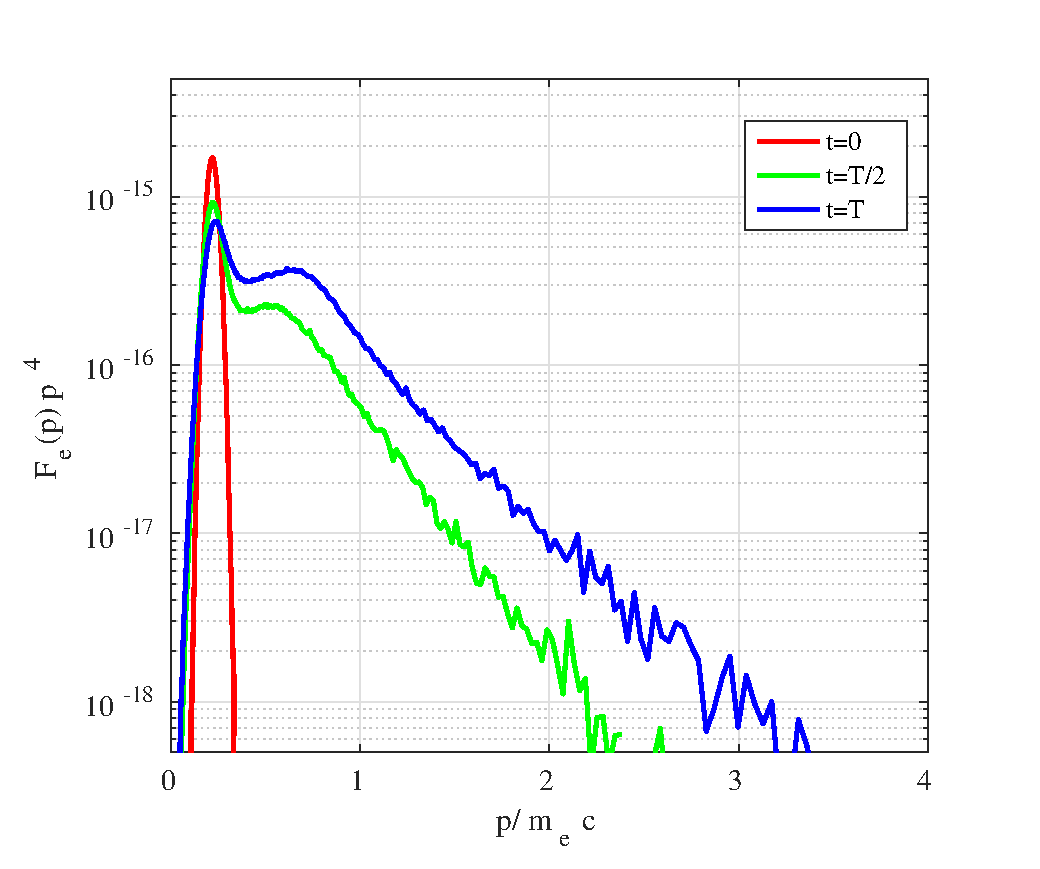
\includegraphics[width=0.8\textwidth]{fig/electrons.eps} 
	\caption{Distribution of electrons.}
	\label{electrons}
\end{figure}

The results presented in Figures \ref{protons}-\ref{electrons_with_alpha} show that the values of $F(p)p^4$ for high energies are much greater for protons, than for electrons in both simulations. Also electrons need much more time to be accelerated and to form spectrum $\propto p^{-4}$. It means that protons are injected into the acceleration process more efficiently, and it is consistent with the work of Park et al. {\cite{Park2015}}. Also we have shown that minority of heavy ions increases the spectrum of protons and do not have influence on the spectrum of electrons. It can be explained by the fact, that heavy ions form the large scale turbulence and protons can efficiently scatter on this turbulence. Otherwise for electrons turbulence produced by protons is already enough large-scale  and the influence of heavy ions is neglectable. 

\section{Conclusions}
In this paper we presented the developed 3D implicit particle-in-cell code, which can be applied for various problems in the collisionless plasma. We have tested it and obtained results, that are consistent with theoretical predictions. We studied the influence of admixture of heavy ions on the evolution of the shock wave and simulations have shown that the presence of heavy ions increases the number of accelerated particles. Further research is necessary in order to study this phenomena in detail.
\ack
A M Bykov, P E  Gladilin and S M  Osipov have developed the implicit fields solver module, which provides conservation of the divergenceless magnetic field. 
V I Romansky acknowledges support from RSF grant 16-12-10519 which was used to develop the
particle mover, parallelization and perform the testing of the code.


The results of the work were obtained using computational resources of Peter the Great Saint-Petersburg Polytechnic University Supercomputing Center (http://www.spbstu.ru).
\section*{References}
\begin{thebibliography}{20}
\bibitem{Bell1978} Bell A R 1978 \textit{MNRAS} \textbf{182} 147
\bibitem{Blandford1978} Blandford R D and Ostriker J P 1978 \textit{Astrophys. J.} \textbf{221} L29 
\bibitem{Berezhko2003} Berezhko E G, Ksenofontov L T and V{\"o}lk H J  2003 \textit{A}{\&}\textit{A} \textbf{412} L11
\bibitem{Uchiyama2007} Uchiyama Y, Aharonian F A, Tanaka T, Takahashi T and Maeda Y 2007 \textit{Nature} \textbf{449} 576
\bibitem{Lapenta2006} Lapenta G, Brackbill J U and Ricci P 2006 \textit{Phys. Plasmas} \textbf{13} 055904
\bibitem{Noguchi2007} Noguchi K, Tronci C, Zuccaro G and Lapenta G 2007 \textit{Phys. Plasmas} \textbf{14} 042308
\bibitem{Weibel1959} Weibel E S 1959 \textit{Phys. Rev. Lett.} \textbf{2} 83
\bibitem{Yoon1987} Yoon P H and Davidson R C 1987 \textit{Phys. Rev. A} \textbf{35} 2718
\bibitem{Park2015} Park J, Caprioli D and Spitkovsky A 2015 \textit{Phys. Rev. Lett.} \textbf{114} 085003
\end{thebibliography}
\end{document}